\documentclass{article}
\usepackage{lipsum}
\usepackage{amsmath}
\usepackage{flafter} 
\usepackage{hyperref}
\usepackage{incgraph}

\begin{document}

\title{Przykładowy dokument}
\author{Jan Kowalski}
\maketitle

\tableofcontents

\section{Section}
\subsection{Subsection}
\subsubsection{Subsubsection}

\lipsum[1-5]

\section{Style tekstów}

Ten tekst jest w \textit{kursywie}, ten jest \underline{podkreślony}, a tamten \textbf{\textit{\underline{ma wszystko na raz}}}!

\section{Środowiska}

\subsection{Listy}

Lista punktowa:
\begin{itemize}
    \item to
    \item jest
    \item lista
\end{itemize}

Lista numerowana:

\begin{enumerate}
    \item to
    \item jest
    \item lista
\end{enumerate}

\subsection{Równania}
Mamy równanie $x^2 = -1$. A co gdybyśmy chcieli napisać inline jakieś ułamki z całeczką np. $\int_{4}^{20} \frac{6}{9} xd$?

Wygląda to marnie. W takiej sytuacji gdy nie przejmujemy się wysokością linii możemy użyć komendy 'limits', dzięki czemu uzyskamy coś takiego $\int\limits_{4}^{20} \frac{6}{9} xd$

Ale to też wygląda dość słabo. Wtedy można pójść na całość i dołożyć 'displaystyle' do komendy 'limits' i uzyskamy coś takiego: $\displaystyle\int\limits_{4}^{20} \frac{6}{9} xd$

O ile równanie wygląda już o wiele lepiej to należy pamiętać o tym, że zajmuje ono więcej miejsca w pionie przez co linijki są o wiele o siebie bardziej oddalone co może negatywnie wpłynąć na czytelność tekstu.

Mamy też niesamowicie ładnie wyglądające równania o takie o:

\begin{equation}
    \sum_{n = 1}^{\infty}  \oint 2137x \, dx = \cos 3x \label{eq:rownanie}
\end{equation}


Do nich możemy się też odnosić \hyperref[eq:rownanie]{1} w tekście.

\subsection{Tabelki}

\begin{table}[]
    \centering
    \caption{Przykładowa tabela}
    \begin{tabular}{|l|l|c|r|}           \hline
              & \textbf{Identifier} & Income & Loses \\ \hline
        $P_1$ & 493                 & 32039  & 30102 \\ \hline
        $P_2$ & 20304               & 25741  & 39122 \\ \hline
        $P_3$ & 93921               & 54039  & 11932 \\ \hline
    \end{tabular}
\end{table}

\pagebreak
\subsection{Obrazki}
\LaTeX pozwala nam na dodawanie obrazków.


\begin{center}
    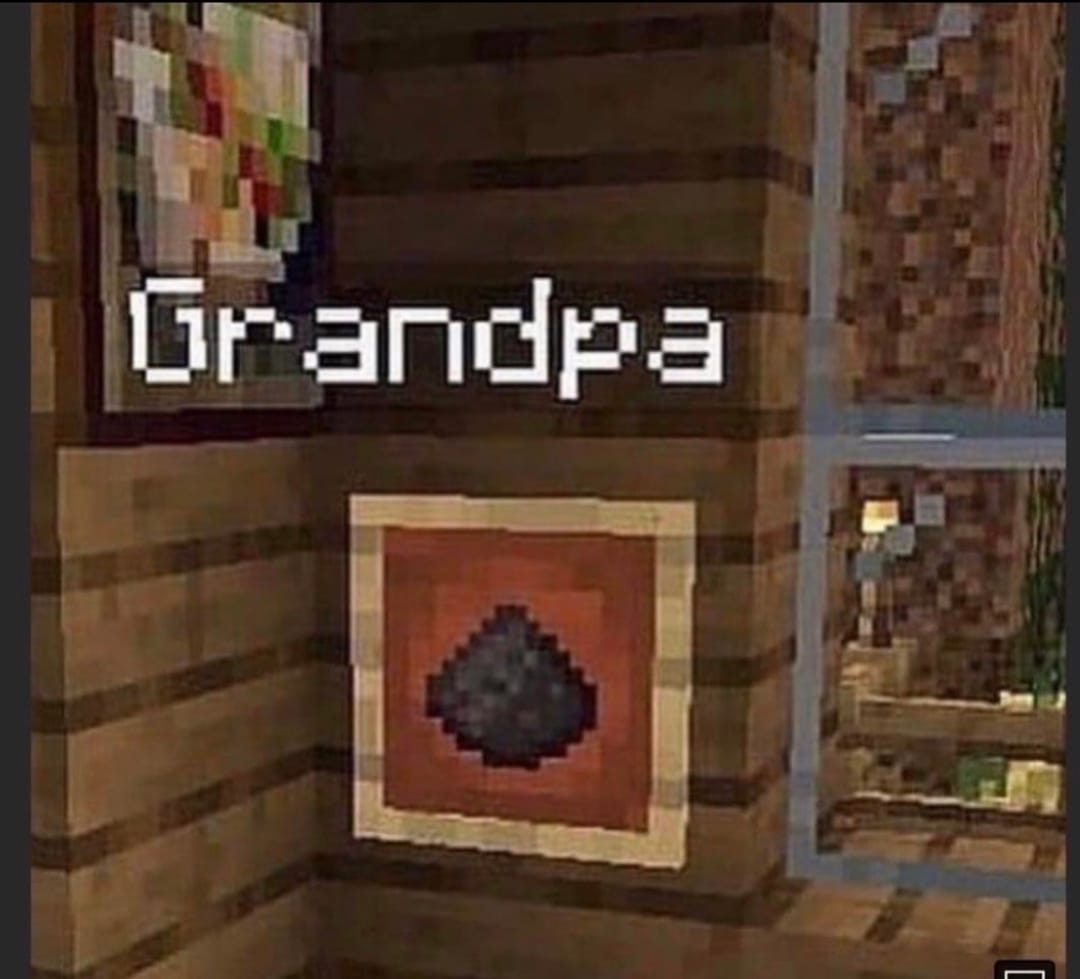
\includegraphics[scale=0.3]{zdjecie.png}
    Tutaj jest przykładowy obrazek \cite{mem}.
\end{center}

\bibliographystyle{plain}
\bibliography{references}

\end{document}
